\documentclass{beamer}
\usepackage[utf8]{inputenc}
\usepackage[T1]{fontenc}
\usepackage[polish]{babel}
\usepackage{graphicx}
\usepackage{times}

\usetheme{AGH}

\title[Biometryczny System Kontroli Dostępu]{Biometryczny System Kontroli Dostępu}

\author[T. Drzewiecki, J. Gajda]{Tomasz Drzewiecki, Joanna Gajda}

\date[2012]{9.01.2012}

\institute[AGH-UST]
{Wydział Elektrotechniki, Automatyki, Informatyki i Elektroniki\\ 
Katedra Automatyki
}

\setbeamertemplate{itemize item}{$\maltese$}

\begin{document}

{
%\usebackgroundtemplate{
\includegraphics[width=\paperwidth]{titlepage}} % wersja angielska
\usebackgroundtemplate{
\includegraphics[width=\paperwidth]{titlepagepl}} % wersja polska
 \begin{frame}
   \titlepage
 \end{frame}
}

%---------------------------------------------------------------------------

\begin{frame}
\frametitle{Tematyka projetku}

\begin{block}{Cel projektu}
Celem naszego projektu było stworzenie/rozbudowa systemu do identyfikacji osób na podstawie tęczówki oka.
\end{block}

\begin{figure}
\begin{center}
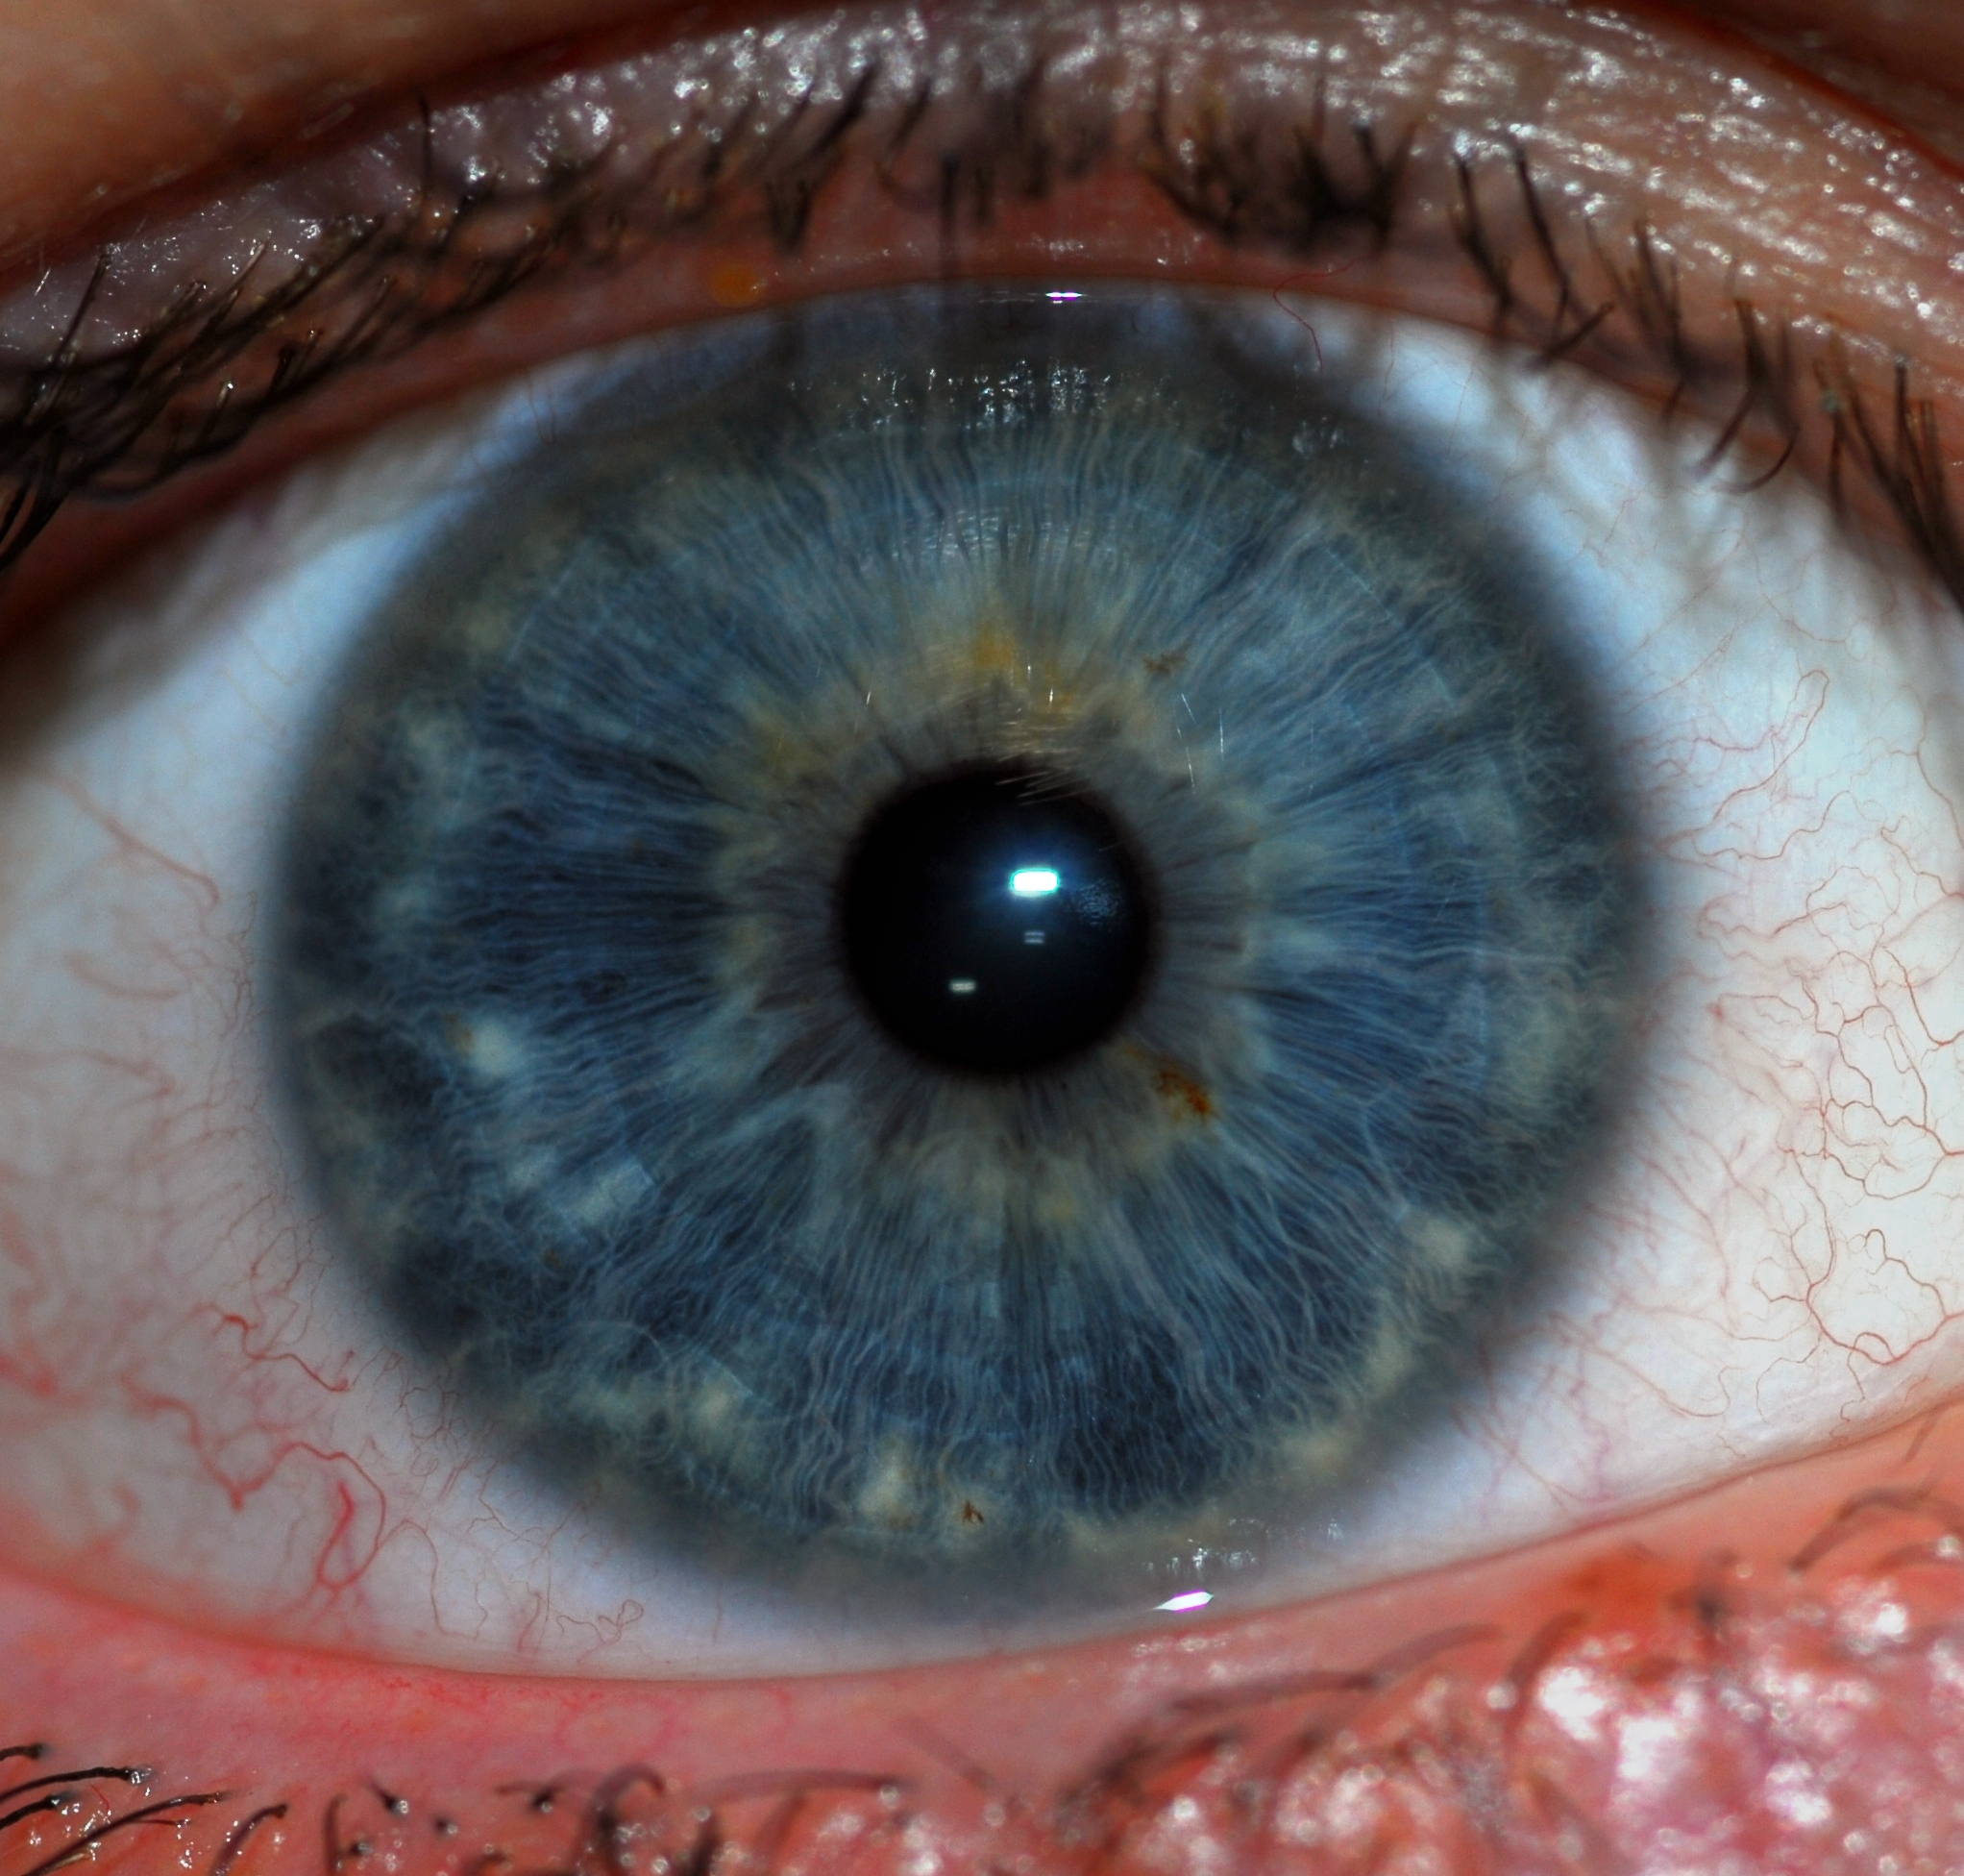
\includegraphics[scale=0.04]{teczowka.jpg}
\caption{Tęczówka człowieka}
\end{center}
\end{figure}

\end{frame}

%---------------------------------------------------------------------------

\begin{frame}
\frametitle{Podział systemu}

Tworzony przez nas system składa się z trzech głównych cześci:
\begin{columns}[t]
\column{0.3\textwidth}
\begin{block}{Część sprzętowa}
Odpowiedzialna za pobranie obrazu tęczówki od badanych osób. Najważniejszym elementem jest kamera oraz zapewnienie odpowiednich warunków.
\end{block}
\column{0.3\textwidth}
\begin{block}{Cześć biometryczna}
Część odpowiedzialna na zamianę obrazu tęczówki na kod tęczówki oraz późniejsze porównywanie utworzonych kodów.
\end{block}
\column{0.3\textwidth}
\begin{block}{Część bazodanowa}
Część odpowiedzialna za przechowywanie danych osób wprowadzanych do systemu.
\end{block}
\end{columns} 

\end{frame}

%---------------------------------------------------------------------------

\begin{frame}
\frametitle{Konstrukcja stanowiska}
Stanowisko do pobierania obrazów musi spełniać odpowiednie wymagania. Im lepsze będą pobierane obrazy, tym łatwiejsza będzie późniejsza segmentacja. Główne założenia:
\begin{itemize}
\item Likwidacja odblasków pochodzących z oświetlenia (naturalnego oraz sztucznego),
\item Odpowiednia jasność obrazu,
\item Odpowiednia jakość obrazu,
\item Odpowiednia wielkość tęczówki na obrazie.
\end{itemize}
\end{frame}
%---------------------------------------------------------------------------

\begin{frame}
\frametitle{Konstrukcja stanowiska}
Udało się skonstruować stanowisko spełniające wymagania:
\begin{itemize}
\item Odblaski usunięto poprzez zasłonięcie źródeł światła (za pomocą kartonowego pudła),
\item Odpowiednią jasność zapewnia oświetlacz IR,
\item Odpowiednią jakość obrazu zapewnia odpowiednia kamera, która potrafi rejestrować obrazy w dużej rozdzielczości,
\item Odpowiednią wielkość tęczówki otrzymujemy stosując przybliżenie za pomocą obiektywu.
\end{itemize}
\end{frame}

%---------------------------------------------------------------------------

\begin{frame}
\frametitle{Stworzone stanowisko}
Kilka zdjęć
\begin{figure}
\begin{center}
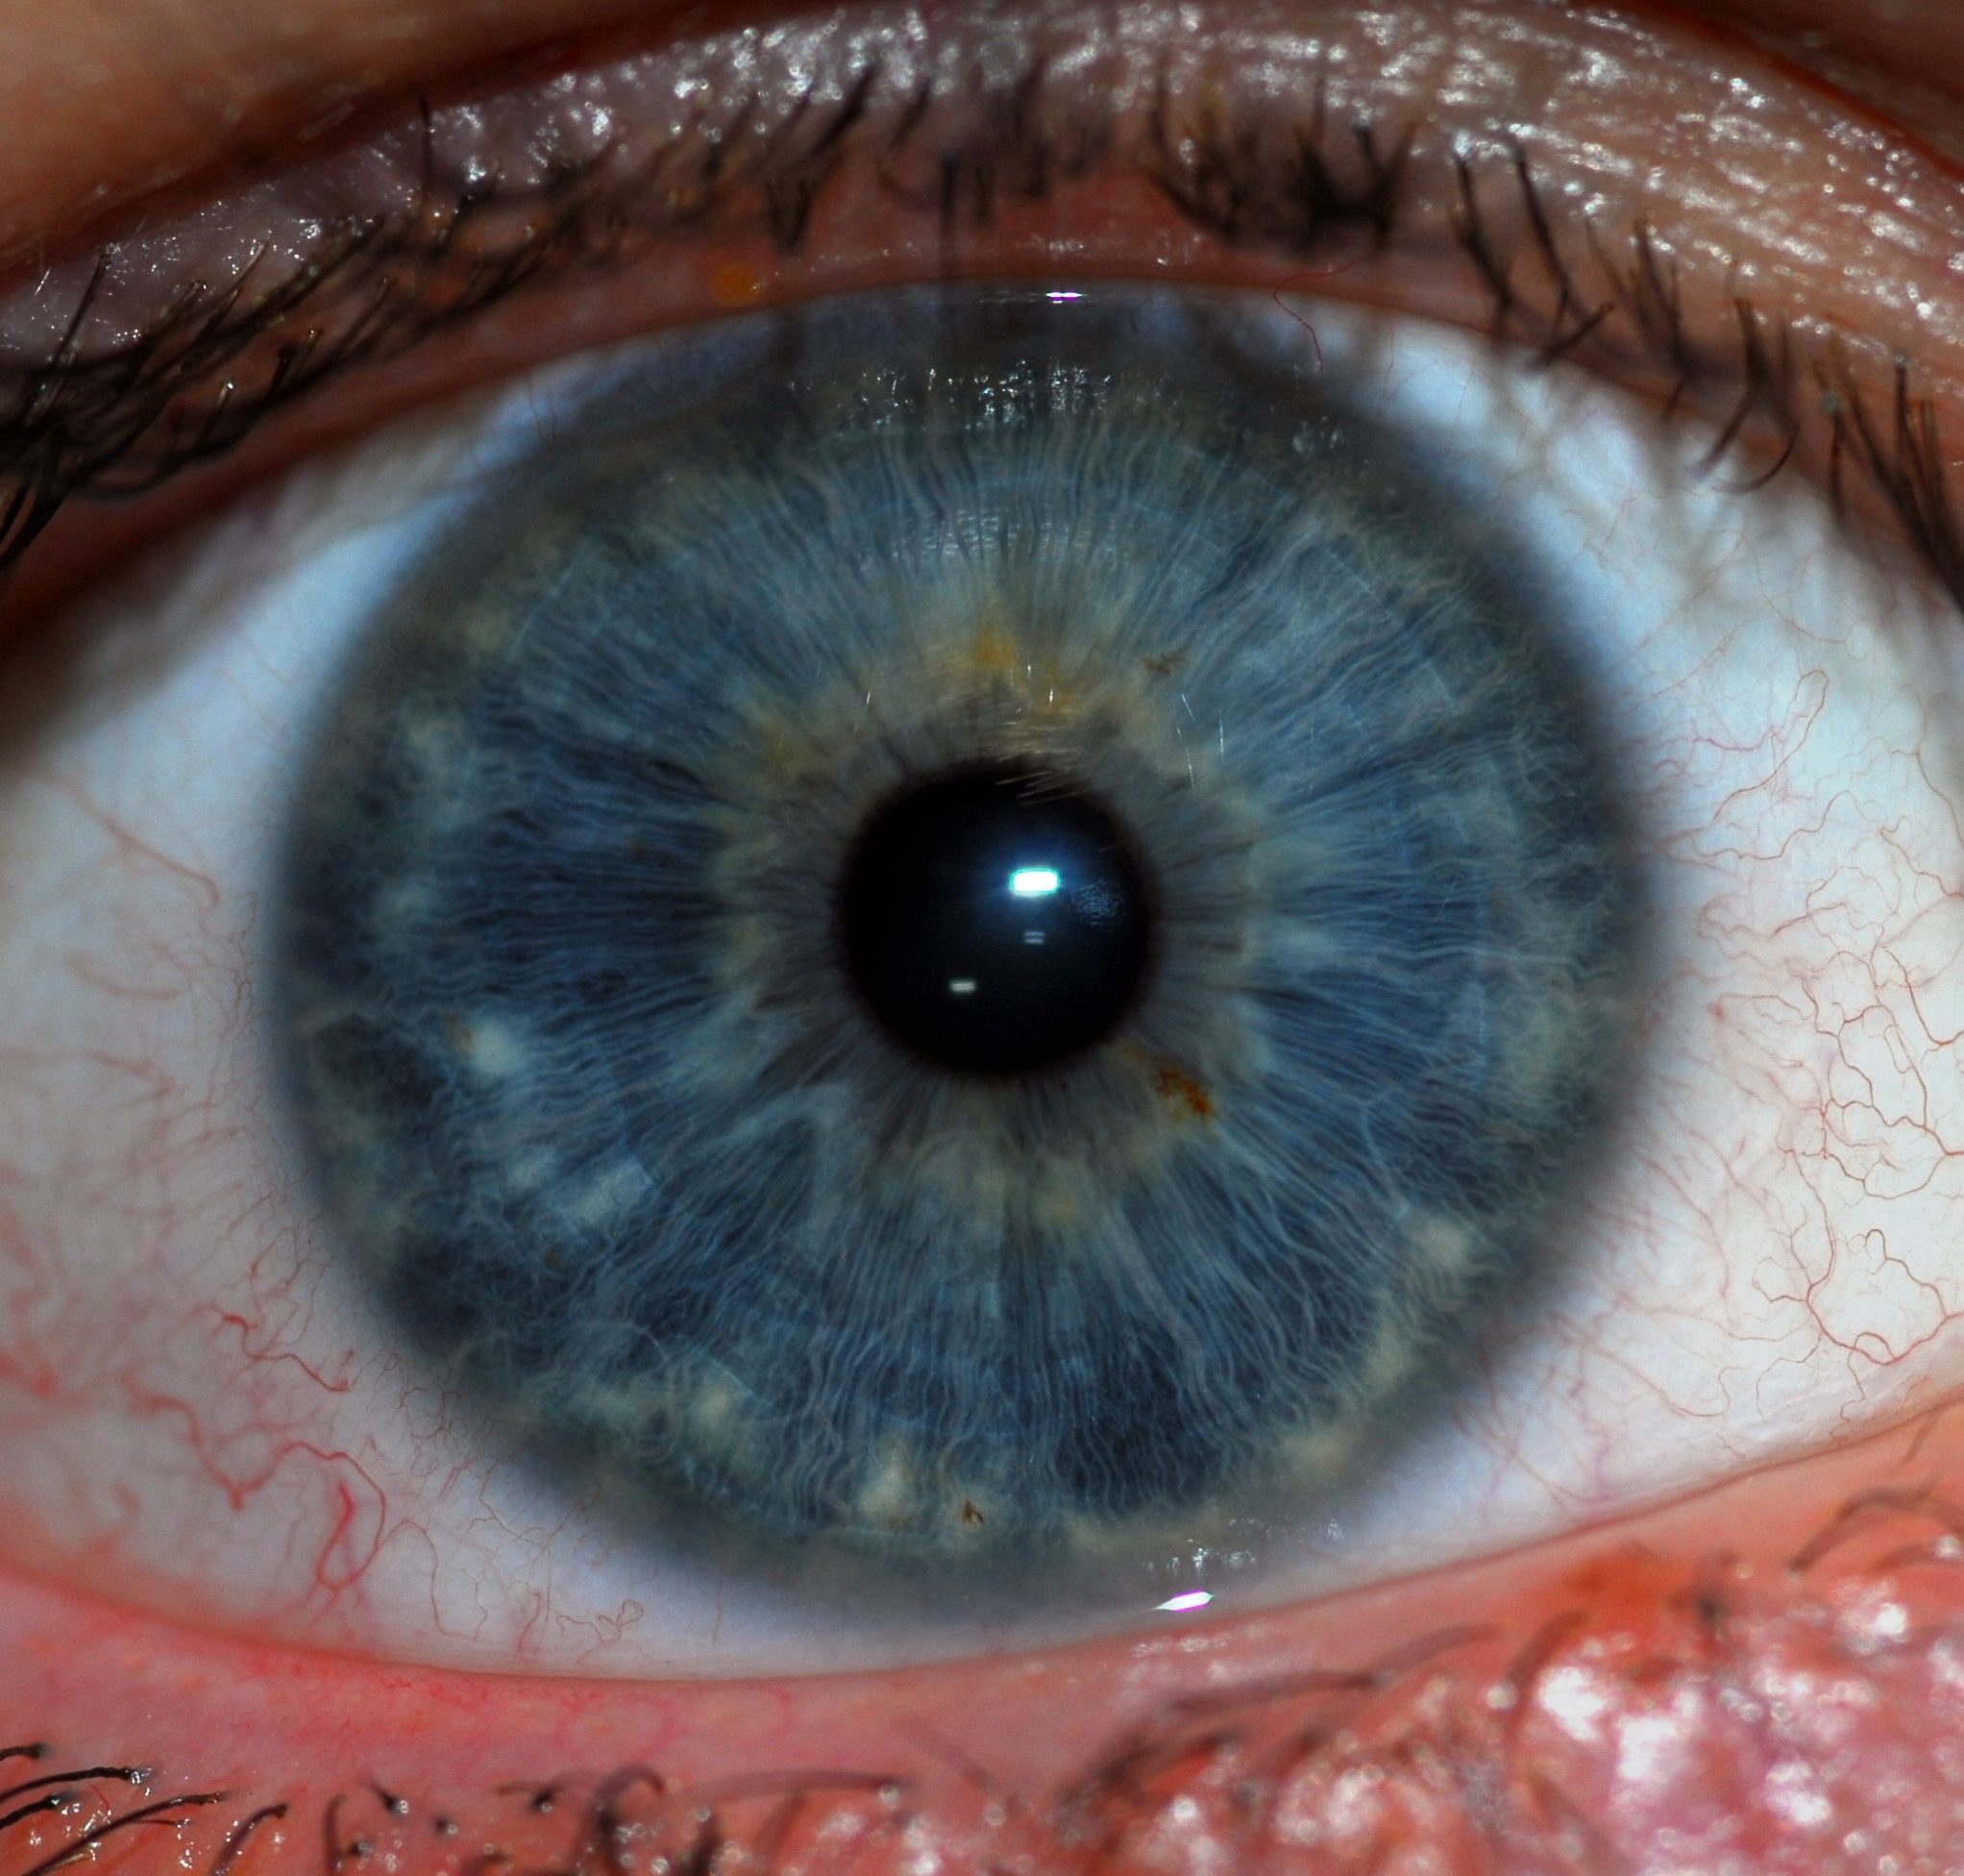
\includegraphics[scale=0.04]{stanowisko.jpg}
\end{center}
\end{figure}
\end{frame}

%---------------------------------------------------------------------------

\begin{frame}
\frametitle{Algorytm do tworzenia kodu tęczówki}
\begin{figure}
\begin{center}
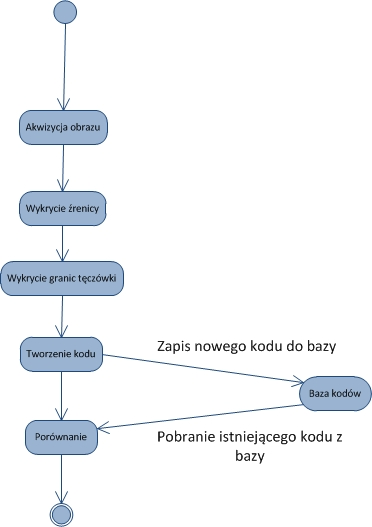
\includegraphics[scale=0.4]{schemat.jpg}
\end{center}
\end{figure}
\end{frame}

%---------------------------------------------------------------------------

\begin{frame}
\frametitle{Wykrycie źrenicy}
Celem tej części algorytmy jest opisanie źrenicy jako okrąg, czyli znalezienie środka okręgu na obrazie oraz jego promienia. Punktem startowym jest pobrany obraz z kamery.
\begin{figure}
\begin{center}
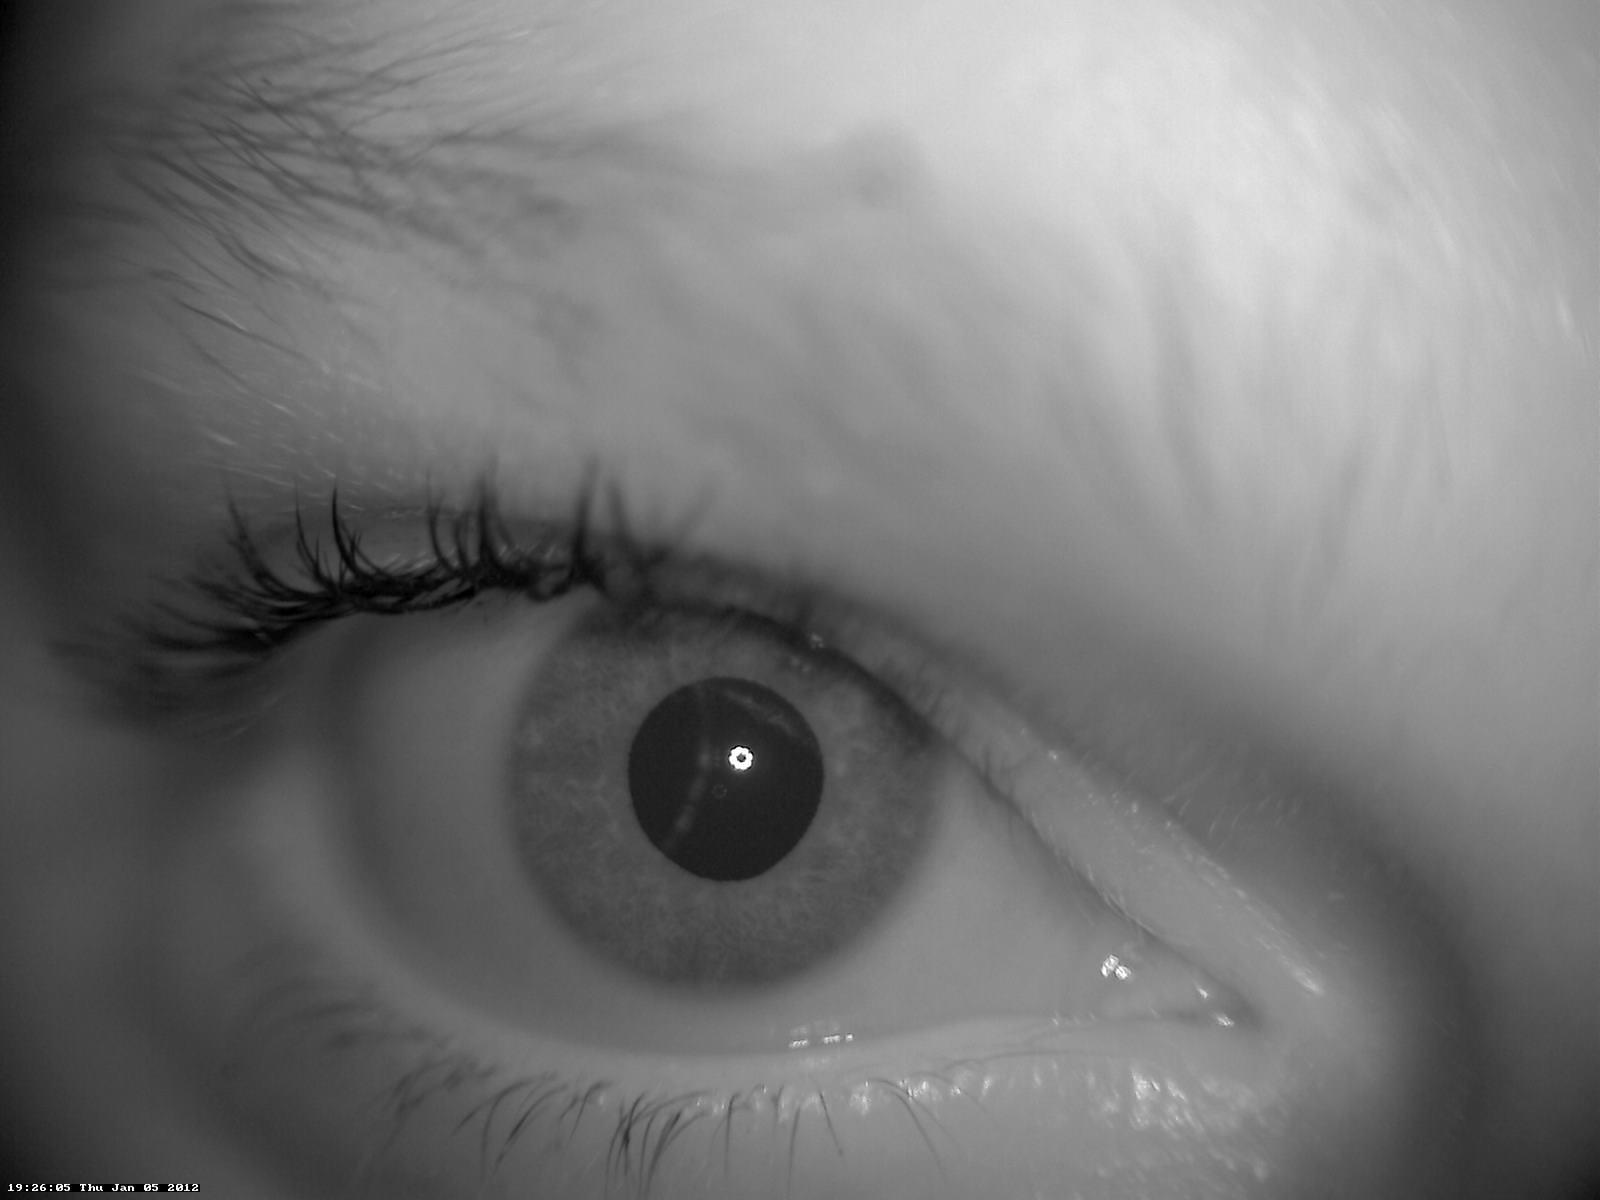
\includegraphics[scale=0.13]{szarosc.jpg}
\end{center}
\end{figure}
\end{frame}

%---------------------------------------------------------------------------

\begin{frame}
\frametitle{Wykrycie źrenicy}
Następnie wyszukiwany jest odblask widoczny na źrenicy i pochodzący od oświetlacza IR. Wyszukiwany jest jasny punkt w otoczeniu ciemnych. Po znalezieniu odblasku do dalszych przekształceń wybierany jest fragment obrazu w jego otoczeniu (kwadrat o boku 220 pikseli z odblaskiem w środku.
\end{frame}

%---------------------------------------------------------------------------

\begin{frame}
\frametitle{Wykrycie źrenicy}
Następnie w wybranym fragmencie obrazu stosujemy operację binaryzacji w celu wyznaczenia źrenicy z dwoma progami: mniejsze od 60 w celu znalezienia pikseli źrenicy oraz większe od 254 w celu znalezienie pikseli odblasku.
\begin{figure}
\begin{center}
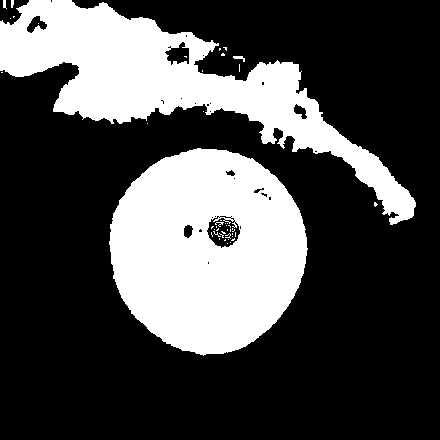
\includegraphics[scale=0.25]{bin.jpg}
\end{center}
\end{figure}
\end{frame}

%---------------------------------------------------------------------------

\begin{frame}
\frametitle{Wykrycie źrenicy}
Kolejno są stosowane operacje zamknięcia i dwukrotnie otwarcia (za drugim razem ze zwiększonym obiektem strukturalnym) w celu otrzymania koła określającego źrenicę.
\begin{columns}
	\column{0.3\textwidth}
		\begin{figure}
		\begin{center}
		
\includegraphics[scale=0.25]{zamkniecie.jpg}
		\end{center}
		\end{figure}
	\column{0.3\textwidth}
		\begin{figure}
		\begin{center}
		
\includegraphics[scale=0.25]{otwarcie1.jpg}
		\end{center}
		\end{figure}
	\column{0.3\textwidth}
		\begin{figure}
		\begin{center}
		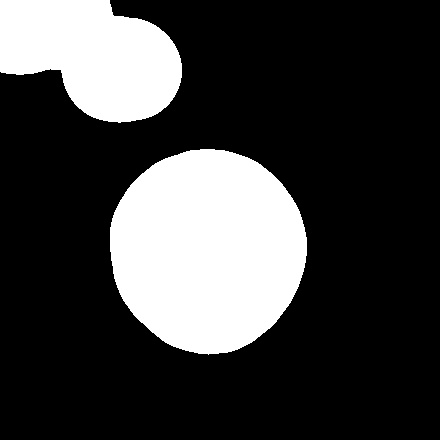
\includegraphics[scale=0.25]{otwarcie2.jpg}
		\end{center}
		\end{figure}
\end{columns}
\end{frame}

%---------------------------------------------------------------------------

\begin{frame}
\frametitle{Wykrycie źrenicy}
Ponieważ na niektórych obrazach po wcześniej wymienionych operacjach pozostaje biały obszar w miejscu, gdzie na obrazie występują rzęsy oraz tym, że ten obszar zawsze jest styczny z brzegiem fragmentu obrazu to stosowany jest algorytm czyszczenia brzegów.
\begin{columns}
	\column{0.5\textwidth}
		\begin{figure}
		\begin{center}
		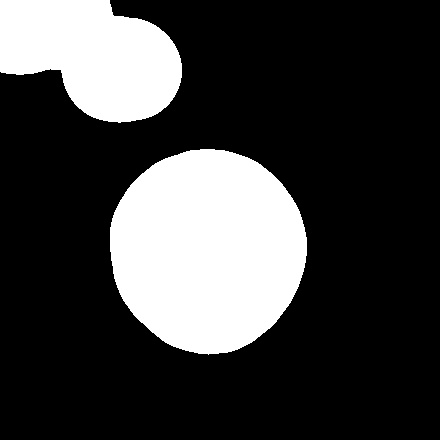
\includegraphics[scale=0.25]{roi1.jpg}
%		\caption{Obraz przed czyszczeniem brzegów}
		\end{center}
		\end{figure}
	\column{0.5\textwidth}
		\begin{figure}
		\begin{center}
		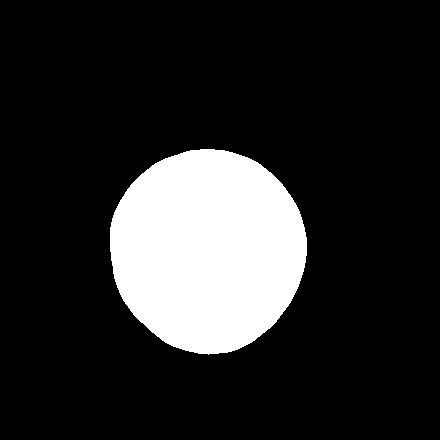
\includegraphics[scale=0.25]{roi2.jpg}
%		\caption{Obraz po czyszczenu brzegów}
		\end{center}
		\end{figure}
\end{columns}
\end{frame}

%---------------------------------------------------------------------------

\begin{frame}
\frametitle{Wykrycie tęczówki}
Sposób wykrywania tęczówki jest zgodny z patentem Daugmana oraz z pracą z poprzedniego roku. Po wykonaniu algorytmu widzimy obszar na zdjęciu, w którym znajduje się tęczówka.
\begin{figure}
\begin{center}
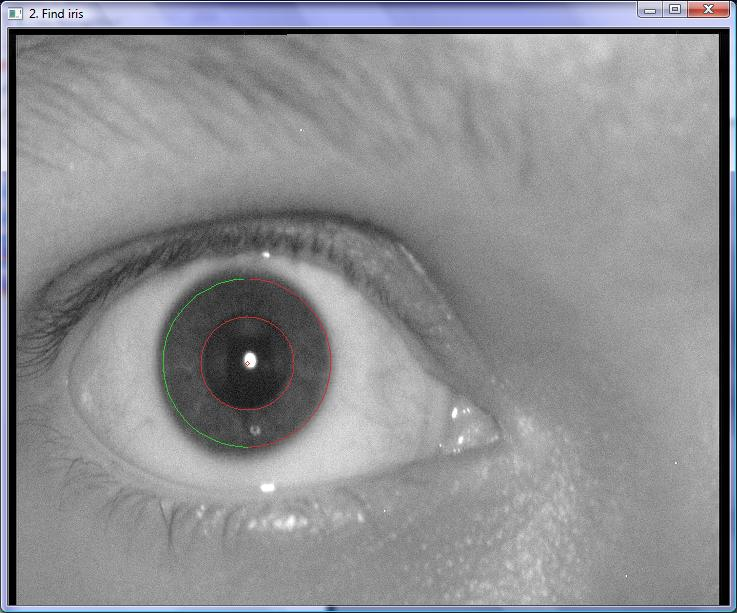
\includegraphics[scale=0.25]{teczowka_nasza.jpg}
\end{center}
\end{figure}
\end{frame}

%---------------------------------------------------------------------------

\begin{frame}
\frametitle{Wykrycie tęczówki}
Sposób wykrywania tęczówki jest zgodny z patentem Daugmana oraz z pracą z poprzedniego roku. Po wykonaniu algorytmu widzimy obszar na zdjęciu, w którym znajduje się tęczówka.
\begin{figure}
\begin{center}
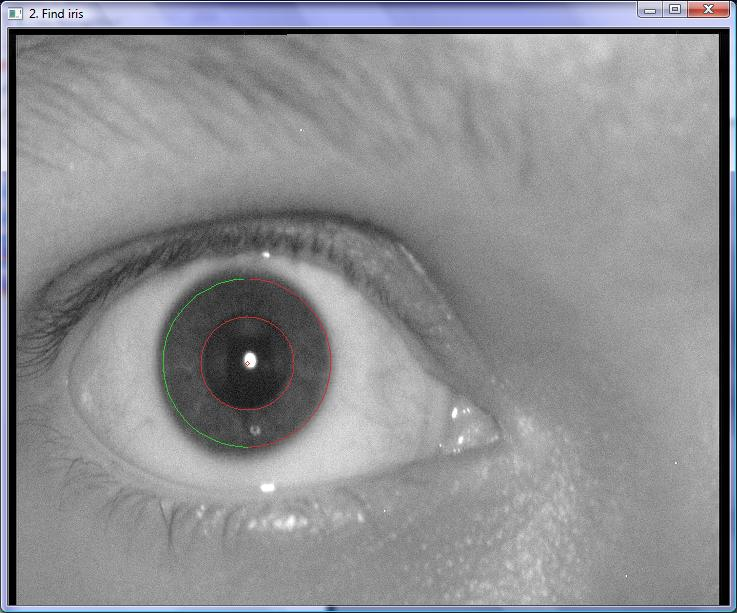
\includegraphics[scale=0.25]{teczowka_nasza.jpg}
\end{center}
\end{figure}
\end{frame}

%---------------------------------------------------------------------------

\begin{frame}
\frametitle{Tworzenie kodu tęczówki}
Kod tęczówki jest tworzony w następujący sposób:
\begin{itemize}
\item Wybieranych jest odpowiednia liczba obszarów, tak aby powstał kod o długości 2048 bitów,
\item Każdy z obszarów jest filtrowany filtrami Gabora (jest ich 8, każdy o innym kierunku),
\item Sumowane są otrzymane liczby zespolone,
\item Koduje się sumy, osobno część rzeczywistą oraz urojoną: 1 dla sumy danej części większej od 0, 0 dla sumy danej części mniejszej lub równej 0.
\end{itemize}
\end{frame}

%---------------------------------------------------------------------------

\begin{frame}
\frametitle{Porównywanie kodów}
Kody porównuje się licząc ile jest różnych pikseli dla dwóch kodów w stosunku do długości kodu. Używany jest wzór:
$$ H = \sum \frac{XOR(A,B)}{2048} $$
gdzie:
$A, B$ - porównywane kody tęczówek, każdy o długości 2048 bitów.\\
\end{frame}

%---------------------------------------------------------------------------

\begin{frame}
\frametitle{Wynik porównania}
Uznaje się, że dwa zdjęcia są zdjęciami jednej tęczówki w przypadku, gdy wyliczona odległość Haminnga ma wartość poniżej 0.18. Jeśli jest równa lub większa to uznaje się, że obrazy przedstawiają różne tęczówki.
\end{frame}

%---------------------------------------------------------------------------

\begin{frame}
\frametitle{Iplementacja}
\begin{itemize}
\item Język C++.
\item Biblioteka do przetwarzania obrazów: OpenCV.
\item Biblioteka do tworzenia interfejsu graficznego: Qt.
\item System zarządzania bazami danych: SQLite.
\end{itemize}
\end{frame}

%---------------------------------------------------------------------------


\begin{frame}
\frametitle{Wyniki i wnioski}
\begin{itemize}
\item Udało się skonstruować system do identyfikacji na podstawie tęczówki.
\item Najważniejsze jest uzyskanie dobrego obrazu, z jak najmniejszą liczbą zakłóceń.
\item Stworzone stanowisko nie jest przenośne.
\item Tęczówka na zdjęciu musi być duża, potrzeba jest dużej liczby szczegółów tęczówki.
\item Najtrudniejszym etapem podczas tworzenia kodu tęczowki jest segmentacja źrenicy.
\end{itemize}
\end{frame}


%---------------------------------------------------------------------------
\begin{frame}
\frametitle{Koniec}

\begin{block}{}
Dziękujemy za uwagę.\\
Pytania?
\end{block}

\end{frame}

%---------------------------------------------------------------------------


\end{document}

